\subsection{Adherence Parameter Accuracy } \label{integr-synth-alpha-sect}
In this experiment, we test if the BCC model can recover the value of the adherence parameter with reasonable accuracy. Since, we have the ground truth values for $\alpha$ from the synthetic data, we can compare them with the estimated $\hat{\alpha}$ returned from the BCC model. \emph{Fig. \ref{adherence-test-pic}} depicts the estimated $\hat{\alpha}$ (on the y-axis) versus the true $\alpha$ (on the x-axis) for the 100 realizations of the synthetic data. For each realization, we show the \emph{mean} value of the estimated $\hat{\alpha}$ together with its $95$\% \emph{credible interval} based on the $2.5 - 97.5$ percentiles of the MCMC simulations. 
\begin{figure}[!ht]
\begin{center}
 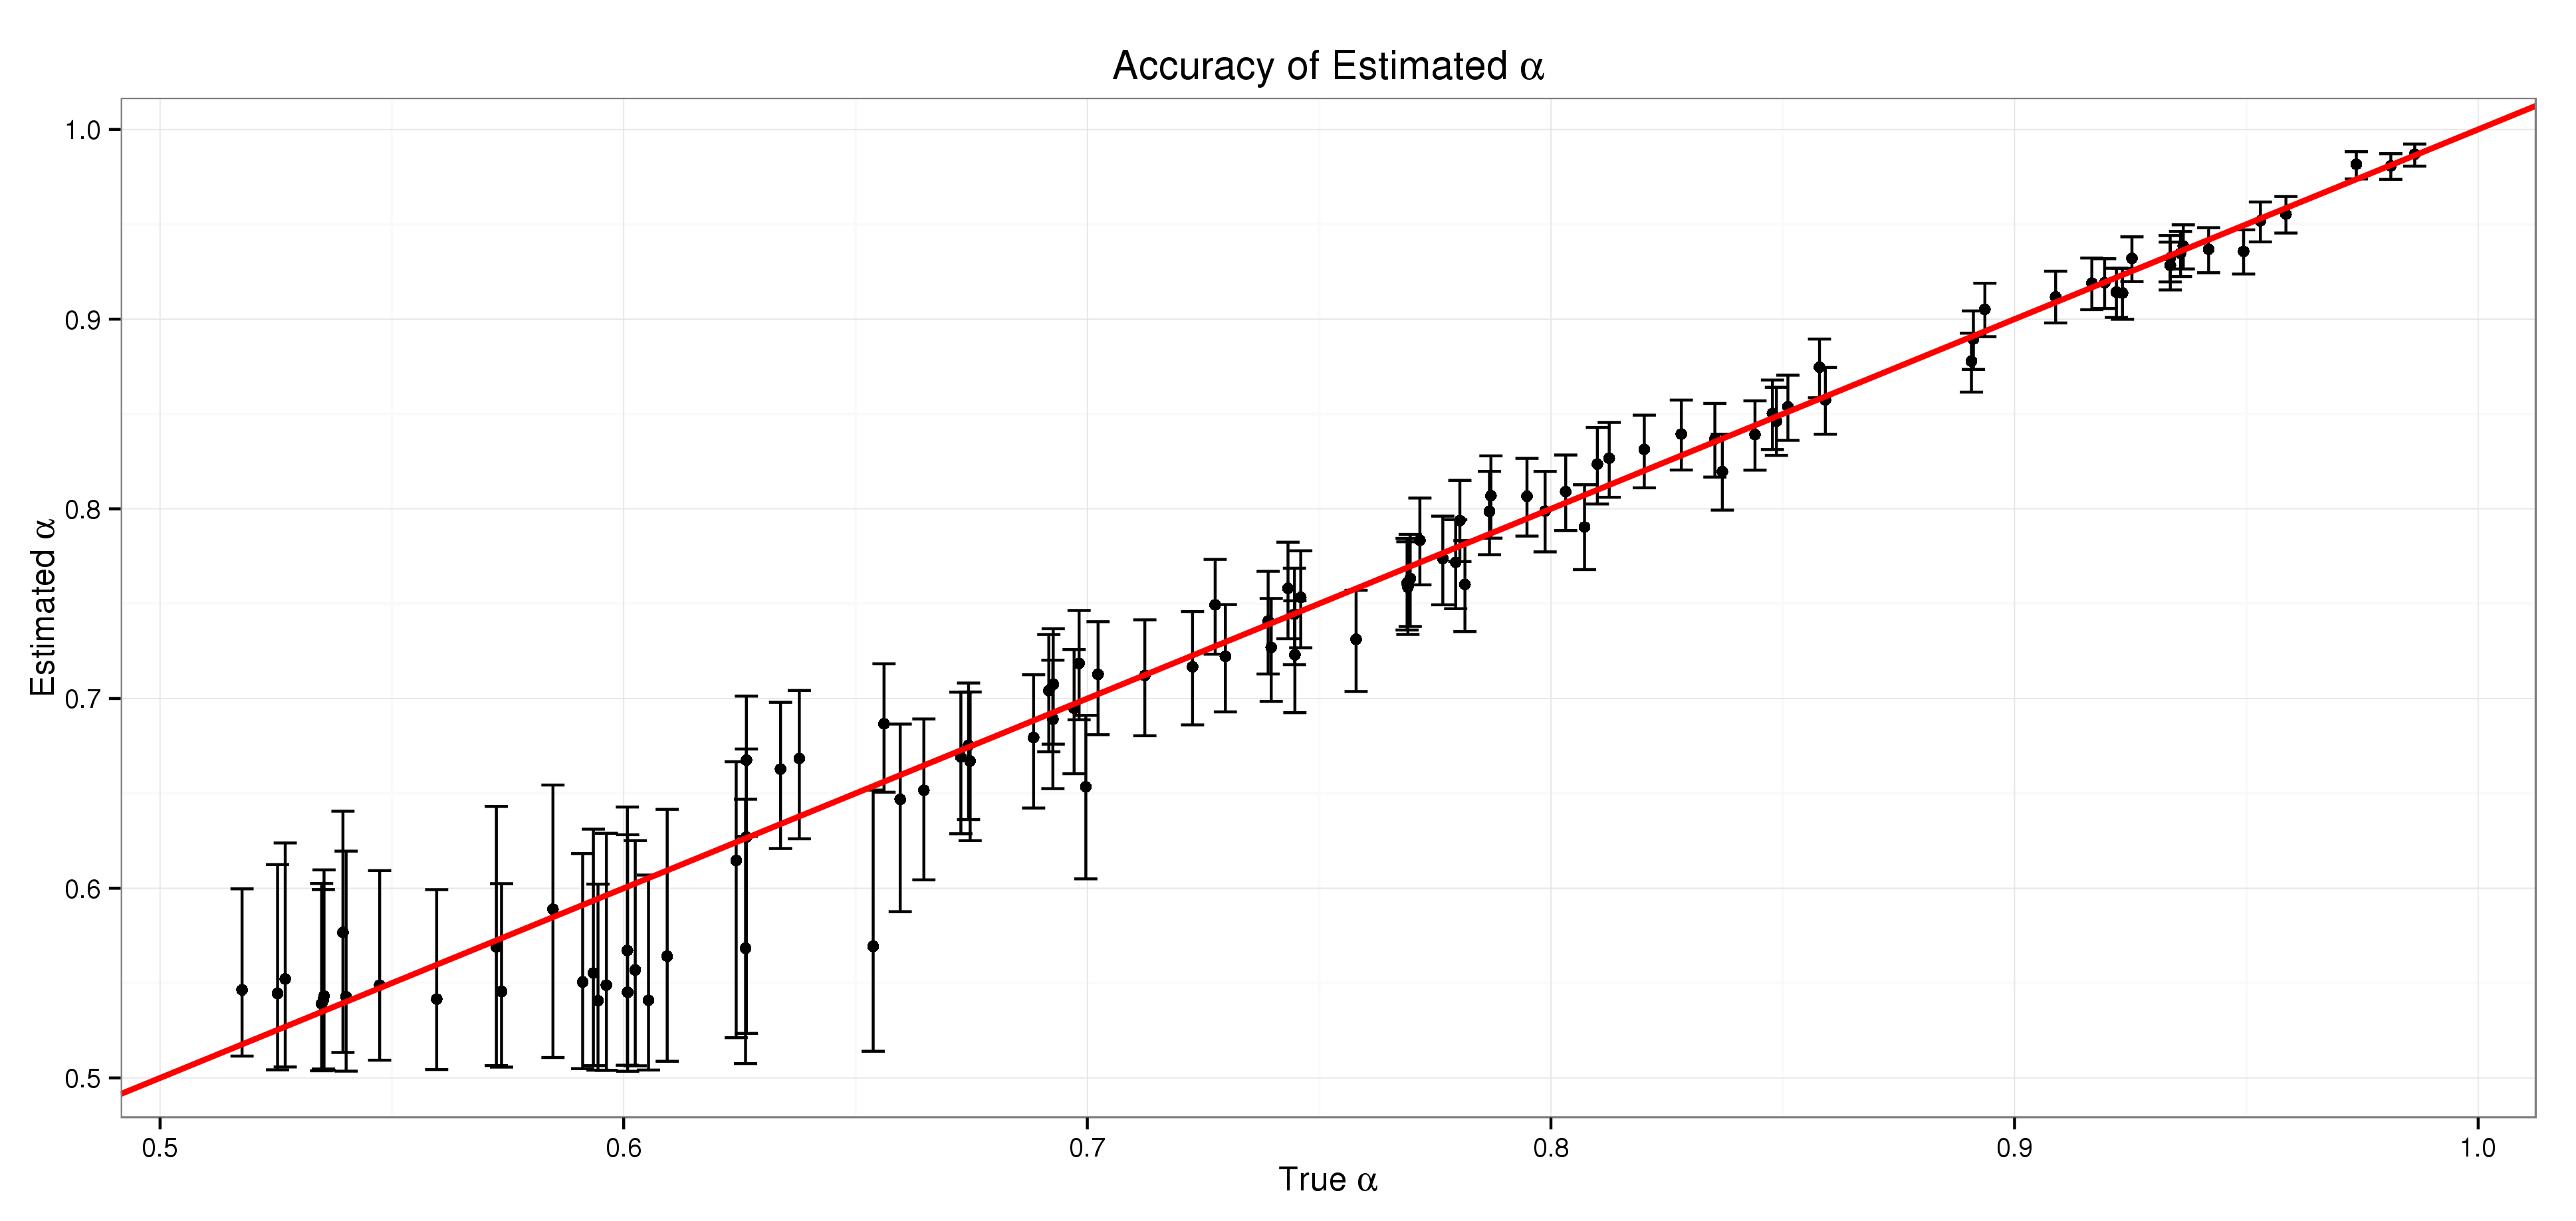
\includegraphics[scale = 0.41]{images/adherenceTest.png}
\caption{\emph{Comparison of estimated $\hat{\alpha}$ (y-axis) versus true $\alpha$ (x-axis) for the 100 realizations of the synthetic data. Values in the main diagonal show perfect agreement. For each realization, the mean value of $\hat{\alpha}$ and the $95$\% credible interval is shown.}}
\label{adherence-test-pic}
\end{center}
\end{figure}

In general, we observe that the true value of $\alpha$ can be recovered with reasonable accuracy, and more specifically in 97 of 100 realizations the $95$\% credible interval contains the true value of $\alpha$. Finally, it should be noted that as $\alpha$ increases, the estimate uncertainty decreases (\ie $95$\% credible interval shrinks), thus the BCC model becomes more accurate. This ... is expected, if we think the role of the adherence parameter, and has the following explanation. 

When $\alpha \approx 1$, it means that there is a perfect agreement between the source-specific and the overall clustering assignments. This implies, that there are clear associations between the data sources, thus we would be able to combine them together without losing predictive power. Intuitively, the problem reduces to performing a single 'joint' clustering which is an easier task, especially for our experiments, where the different clusters are well separated. On the other extreme, when $\alpha \approx 0.5$, there is no agreement and any association between the data sources could be random. This is similar to performing a separate clustering on each data source followed by post-hoc integration, but since there are no common features between the data sources, overall clustering assignments could be due to chance, that is why the model has higher variability and also makes less accurate predictions. 